\documentclass{book}

\usepackage[margin=1.3in]{geometry}
\usepackage{amsmath}
\usepackage{amssymb}
\usepackage{epigraph}
\usepackage{titlesec}
\usepackage{color}
\usepackage{longtable}
\usepackage[toc,page]{appendix}
\usepackage{paralist}
\usepackage{cleveref}
\usepackage{transparent}
\usepackage{multirow}
\usepackage[many]{tcolorbox}

\usepackage{tikz}
\usetikzlibrary{positioning}

\definecolor{defgreen}{RGB}{95,174,87}
\definecolor{egblue}{RGB}{35, 104, 99}
\definecolor{thred}{RGB}{167, 56, 62}

\newtcolorbox{defbox}[1][]{
    width=0.9\textwidth,
    arc=0mm,
    colback=defgreen!10,
    colframe=defgreen!0
}
\newtcolorbox{thmbox}[1][]{
    width=0.9\textwidth,
    arc=0mm,
    colback=thred!10,
    colframe=thred!0
}
\newtcolorbox{egbox}[1][]{
    width=0.9\textwidth,
    arc=0mm,
    colback=egblue!10,
    colframe=egblue!0
}

\newcommand{\RR}{\mathbb{R}}
\newcommand{\ZZ}{\mathbb{Z}}
\newcommand{\QQ}{\mathbb{Q}}
\newcommand{\CC}{\mathbb{C}}
\newcommand{\NN}{\mathbb{N}}
\newcommand{\suchthat}{\text{ s.t. }}
\newcommand{\lcm}{\text{lcm}}
\newcommand{\sgn}{\text{sgn}}

\newcommand{\normal}{\triangleleft}
\newcommand{\fgroup}[2]{{\raisebox{.2em}{$#1$}\left/\raisebox{-.2em}{$#2$}\right.}}

\DeclareRobustCommand\iff{\Leftrightarrow}
\DeclareRobustCommand\implies{\Rightarrow}

\newcommand{\deft}[1]{\color{defgreen} \textbf{#1}}
\newcommand{\egft}[1]{\color{egblue} \textbf{#1}}
\newcommand{\thmft}[1]{\color{thred} \textbf{#1}}



\newcounter{definition}[section]
\newenvironment{definition}[1]
{
    \refstepcounter{definition}
    \begin{center}
    \begin{defbox}
    \textbf{\deft{\underline{Definition \thesection.\thedefinition} #1}}\\
}
{
    \end{defbox}
    \end{center}
}

\newcounter{example}[section]
\newenvironment{example}[1]
{
    \refstepcounter{example}
    \begin{center}
    \begin{egbox}
    \textbf{\egft{\underline{Example \thesection.\theexample} #1}}\\
}
{
    \end{egbox}
    \end{center}
}

\newcounter{theorem}[section]
\newenvironment{theorem}[1]
{
    \refstepcounter{theorem}
    \begin{center}
    \begin{thmbox}
    \textbf{\thmft{\underline{Theorem \thesection.\thetheorem} #1}}\\
}
{
    \end{thmbox}
    \end{center}
}

\newenvironment{corollary}
{
    \begin{center}
    \begin{thmbox}
    \textbf{\thmft{\underline{Corollary to \thesection.\thetheorem}}}
}
{
    \end{thmbox}
    \end{center}
}

\newenvironment{proof}
{
    \begin{quote}
    \textit{\textbf{Proof: }}
}
{
\noindent\\ \hspace*{\fill}$\blacksquare$
\end{quote}
}

\title{Undergraduate Mathematics}
\date{}
\author{Steven Rosendahl}

\begin{document}
\maketitle

\tableofcontents{}

\part{Algebra}

\chapter{Proofs and Set Theory}
\section{Logic}

We will begin by introducing the ideas of sets and proof simultaneously. Logic is the fundamental basis of all of mathematics; sets are the building blocks of all the structures that we know and love. There are various ways to prove the assertions in mathematics, but we will start by laying out basic logic rules and definitions. Much of the content of this section is a simplification of the actual logic we will use when proving important mathematical results; in other words, we won't see many truth tables in other chapters and sections. Nonetheless, the topics are fundamental and help us to put the rest of the content of this book into perspective. We will begin with a few definitions. This section will be a little heavy on the definitions as well as notation, but then again, all of mathematics is.

\subsection{Logical Rules}
Let's start off with the fundamental definition of this section.

\begin{definition}{\deft{Statement}}
	A statement is an assertion that is either true or false.
\end{definition}

This may seem like a useless definition, but it actually points out a key fact that we will rely on for the rest of this book; that is, assertions are either true or false. Interestingly, there is a branch of mathematics that deals with statements that can be neither true nor false (often called \textit{multilogic}), but the ideas perpetuated by that field of study exceed the level of material covered here. The state of a statement is known as its truth value.

\begin{definition}{\deft{Truth Value}}
	The truth value of a statement is either true or false.
\end{definition}

Again, this definition is probably intuitive, but ultimately necessary. We typically name a statement $P$. With this in mind, we can begin to look at discrete logical statements. The general idea here is to take two logical statements, typically called $P$ and $Q$, and perform some sort of operation on them. We can think of it like performing operations on numbers; the only difference here is that we have two options, True ($T$) or False ($F$), as opposed to, say, some real number. The following are the four most common operations in the world of logic.

\begin{definition}{\deft{Negation}}
	The negation of a statement $P$, denoted $\neg P$, is the statement that has the opposite truth value of $P$.
\end{definition}
\begin{definition}{\deft{Conjunction}}
	Let $P$ and $Q$ be statements. The conjunction of statements $P$ and $Q$ is the truth value of $P$ and $Q$, denoted $P \land Q$.
\end{definition}
\begin{definition}{\deft{Disjunction}}
	Let $P$ and $Q$ be statements. The disjunction of statements $P$ and $Q$ is the truth value of either $P$ or $Q$, or $P$ and $Q$, denoted $P \lor Q$.
\end{definition}
\begin{definition}{\deft{Implication}}
	Let $P$ and $Q$ be statements. The implication of statements $P$ and $Q$ is the truth value of $P$ implying $Q$, denoted $P\implies Q$.
\end{definition}

These definitions are rather vague; the main purpose of pointing them out is to allow us to become familiar with the notation. Of more importance is the truth table created by the statements. A truth table is a handy way to determine the truth value of the four definitions given the truth values of $P$ and $Q$. The following is a truth table for the negation, conjunction, disjunction and implication of statements $P$ and $Q$. We will follow the convention set by most other mathematics textbooks: $T$ means \textit{true} and $F$ means \textit{false}.

\begin{center}
	\begin{tabular}{c | c | c | c | c | c | c}
		$P$ & $Q$ & $\neg P$ & $\neg Q$ & $P \land Q$ & $P \lor Q$ & $P \implies Q$ \\
		\hline
		$T$ & $T$ & $F$      & $F$      & $T$         & $T$        & $T$       \\
		$T$ & $F$ & $F$      & $T$      & $F$         & $T$        & $F$       \\
		$F$ & $T$ & $T$      & $F$      & $F$         & $T$        & $T$       \\
		$F$ & $F$ & $T$      & $T$      & $F$         & $F$        & $T$       \\
	\end{tabular}
\end{center}

The truth table above is very useful and probably worth memorizing. The only caveat is the implication. The truth values for $P\implies Q$ makes sense, however; if we assert that something is true, it cannot make sense to say that whatever follows is false. In other words statements like \textit{If Alicia is mortal, then she is a dog} do not make sense logically. Let's take a look at some example of creating truth tables.

\begin{example}{\egft{Determine the truth table for the statement $P\land\neg P$}}\label{eg:fallacy}
	In order to show the steps, we will determine the truth values for $P$, $\neg P$, and $P\land\neg P$ individually.
	\begin{center}
		\begin{tabular}{c | c | c}
			$P$ & $\neg P$ & $P\land\neg P$ \\
			\hline
			$T$ & $F$      & $F$\\
			$F$ & $T$      & $F$
		\end{tabular}
	\end{center}
    Here, we have a statement that is always false. Such a statement is called a contradiction. Contradictions will be of great use to us later when we look at proof techniques.
\end{example}

\begin{example}{\egft{Determine the truth table for the statement $P\lor \neg P$}}\label{eg:tautology}
    \begin{center}
		\begin{tabular}{c | c | c}
			$P$ & $\neg P$ & $P\lor\neg P$ \\
			\hline
			$T$ & $F$      & $T$\\
			$F$ & $T$      & $T$
		\end{tabular}
	\end{center}
    This is the opposite of what we had in \cref{eg:fallacy}, and is called a tautology.
\end{example}

At this point, you may be wondering what happens if $P = Q$. We call this

\begin{definition}{\deft{Logical Equivalence}}
	Let $P$ and $Q$ be logical statements. We say $P$ is logically equivalent to $Q$ if the truth values of $P$ and $Q$ are the same. We use the notation $P\equiv Q$.
\end{definition}

\noindent We now have all we need to perform our first true proof. It turns out that truth tables can be used to show logical equivalence of two statements. Consider the following example.

\begin{example}{\egft{Determine if $\neg(P \land Q) \equiv (\neg P \lor \neg Q)$}}\label{eg:demorgan}
	We can use a truth table to prove this result. We will do this by list all possible combinations of $P$ and $Q$, and then determine the truth values of the statements. If the truth values of $\neg(P \land Q)$ and $(\neg P \lor \neg Q)$ are equivalent, we will have shown that the statements are logically equivalent.
	\begin{center}
		\begin{tabular}{c | c | c | c}
			$P$ & $Q$ & $\neg(P \land Q)$ & $(\neg P \lor \neg Q)$ \\
			\hline
			$T$ & $T$ & $F$               & $F$                    \\
			$T$ & $F$ & $T$               & $T$                    \\
			$F$ & $T$ & $T$               & $T$                    \\
			$F$ & $F$ & $T$               & $T$
		\end{tabular}
	\end{center}
	Thus, we conclude that $\neg(P \land Q) \equiv (\neg P \lor \neg Q)$.
\end{example}

The result of \cref{eg:demorgan} is actually a very important result known as DeMorgan's Law. The actual statement of the law is our first theorem.

\begin{namedtheorem}[DeMorgan's Law]\label{thm:demorgan}
	Let $P$ and $Q$ be statements. Then
	\[\neg(P \land Q) \equiv (\neg P \lor \neg Q),\] and
	\[\neg(P\lor Q)\equiv (\neg P \land \neg Q).\]
\end{namedtheorem}

DeMorgan's law is a very powerful mathematical theorem (we will define what a theorem is later) that we will use when proving results about sets. We won't prove the second statement in DeMorgan's law here (see problem \ref{prob:demorgan}), so you can take it for granted here.

Before we finish this section, we will introduce a few more logical operators and their truth tables. The first operator will look similar to disjunction, but with a small change (see problem \ref{prob:xor}).

\begin{definition}{\deft{Exclusive Disjunction}}
	The exclusive disjunction of logical statements $P$ and $Q$ is the disjunction of $P$ and $Q$ where if $P$ and $Q$ are true, then the exclusive disjunction is false. In other words,
	\begin{center}
		\begin{tabular}{c | c | c}
			$P$ & $Q$ & $P\oplus Q$ \\
			\hline
			$T$ & $T$ & $F$         \\
			$T$ & $F$ & $T$         \\
			$F$ & $T$ & $T$         \\
			$F$ & $F$ & $F$
		\end{tabular}
	\end{center}
\end{definition}

The exclusive disjunction, often referred to as \textit{exclusive or} or \textit{xor}, is not as useful as the next logical operator.

\begin{definition}{\deft{Biconditional Implication}}
	Let $P$ and $Q$ be statements. Then the biconditional implication of $P$ and $Q$ is the statement $(P\implies Q)\land(Q\implies P)$, denoted $P\iff Q$.
\end{definition}

The biconditional is often referred to by \textit{if and only if}, or, since mathematicians don't like to write a lot, \textit{iff}. This is a very powerful tool since it allows us to evaluate implication in both directions; it is also a slight annoyance, since we will have to prove both direction of statements that contain \textit{iff}.

\subsection{Quantifiers}

Thus far, we've dealt with only single statements $P$ and $Q$. This is a luxury; we are usually dealing with what is known as an
\begin{definition}{\deft{Open Sentence}}
    An open sentence is a statement with one or more variables that come from a prescribed collection of possible variables. The is written as $P(x)$ where $x$ is within the collection of possible values.
\end{definition}
We now have statements that can take on different values based on the value provided. For example, consider the living creatures within Emily's household as the collection, and the statement $P(x)= x$ is a human. We can ask $P(\text{Emily})$, and we will find that the value is $T$. However, if we ask $P(\text{Rex})$ where Rex is Emily's dog, then the statement is false. Hence, there are \textit{some} living creatures in Emily's household that are humans, and some that are not. Now suppose Emily is a wealthy entrepreneur who own an animal shelter. When the shelter closes, we can ask $Q(x)=x$ is a dog. In this case, we will find that when no humans are in the shelter, there are only dogs, so $Q(x)=T$ \textit{for all} $x$ in the shelter. This leads us to the concept of quantifiers.

\begin{definition}{\deft{Universal Quantifier}}
    Let $P(x)$ be an open sentence and let the collection of allowed values of $x$ be called $S$. The universal quantifier is the allowance of all $x$ to produce $P(x)=T$. In other words, the statement $P(x)=T$ for every $x$ in $S$. We use the symbol $\forall$.
\end{definition}

\begin{definition}{\deft{Existential Quantifier}}
    Let $P(x)$ be an open sentence and let the collection of allowed values of $x$ be called $S$. The existential quantifier, $\exists$, is the allowance of at least one $x$ in $S$ to produce $P(x)=T$. In other words, $P(x)=T$ for at least one $x$ in $S$.
\end{definition}

% TODO -- is this right?
Note that it is possible that neither quantifier applies. In that case, we simply say there is no $x$ that works. Quantifiers can also be negated; the negation of $\forall$ is $\exists$ and the negation of $\exists$ is $\forall$.


\newpage

\section{Set Theory}
Up to now, we have been skating around the idea of what is formally known as a set. We talked about using logical quantifiers, but $\forall$ and $\exists$ only make sense when we have a collection to talk about. Such a collection is called a

\begin{definition}{\deft{Set}}
	A set is a collection of objects called elements.
\end{definition}

This is perhaps one of the simplest definitions that we will ever see; at the same time, it is also one of the most fundamental ideas in mathematics. We can create sets of anything: numbers, functions, and even other sets. They can be finite or infinite, countable or uncountable, etc. Typically, we write sets using \textit{set notation}:
\begin{gather*}
	A = \{a,b,c,d,\dots\},\text{ read as \textit{A is the set containing $a,b,c,d,\dots$}}\\
	A = \{x : P(x)\},\text{ read as \textit{A is the set of $x$ such that $P(x)$ is true}}.
\end{gather*}
Sometimes, we will see a $|$ in place of $:$.

The purpose of this section is to introduce the concept of sets as well as the operations we can perform on sets themselves. Much of the material will parallel that which we've already seen when talking about logic. Let's look at some special sets.

\subsection*{Special Sets}

\begin{definition}{\deft{Empty Set}}
	The empty set is the set with no elements, written as $\emptyset=\{\}$. The empty set is a subset of every set.
\end{definition}
\begin{definition}{\deft{Universal Set}}
	The universal set is the set of which all sets are a subset, typically written as $\mathcal{U}$.
\end{definition}
The universal set leads us into our next concept. It is common in mathematics to define some sort of structure, like a set, and then talk about a substructure, in this case called a subset.
\begin{definition}{\deft{Subset}}
	Let $A$ be a set. Then $B$ is a subset of $A$, written $B\subset A$, if and only if $x\in B\implies x\in A\ \forall x\in B$. Every set is a subset of itself.
\end{definition}
When we want to show something is a subset, we must show that it satisfies this property. We can perform a simple proof using truth tables of this.

\begin{example}{\egft{Show that $\{1,2,3\}\subset\{-1,0,1,2,3\}$.}}
	Let $P(x)$ be the statement \textit{$x$ is in $\{1,2,3\}$} and $Q(x)$ be the statement \textit{$x$ is in $\{-1,0,1,2,3\}$}. We need to show that $P(x)\implies Q(x)$ for each x in $\{1,2,3\}$. Let's layout a truth table.
	\begin{center}
		\begin{tabular}{c | c | c | c}
			$x$ & $P(x)$ & $Q(x)$ & $P(x)\implies Q(x)$ \\
			\hline
			1   & $T$    & $T$    & $T$            \\
			2   & $T$    & $T$    & $T$            \\
			3   & $T$    & $T$    & $T$
		\end{tabular}
	\end{center}
	Therefore, we conclude $\{1,2,3\}\subset\{-1,0,1,2,3\}$.
\end{example}
That was a very simple example since the sets were small and finite, but what if we have an infinite set? Here are some very common sets that we will see repeatedly throughout this book.
\begin{align*}
	\text{Natural Numbers: } & \NN = \{1,2,3,4,\dots\}                    \\
	\text{Integers: }        & \ZZ = \{\dots,-3,-2,-1,0,1,2,3,\dots\}     \\
	\text{Rationals: }       & \QQ = \left\{\frac{a}{b}:a,b\in\ZZ\right\} \\
	\text{Real Numbers: }    & \RR                                        \\
	\text{Complex Numbers: } & \CC = \{a+bi : a,b\in\RR\}
\end{align*}
Note that we did not define the reals. The definition requires a lengthy discussion that cannot be boiled down to a simple set definition. Simply put, it is all of $\QQ$ and everything else that is not in $\QQ$ up to $\CC$; so numbers like $\pi$ and $e$ are in $\RR$. The complex numbers are also a mysterious set that require a lot of time to understand in great detail. These sets have a special relationship, namely:
\[
	\NN\subset\ZZ\subset\QQ\subset\RR\subset\CC.
\]
This list is certainly not comprehensive either. There are sets that exist above $\CC$ and sets that exist between $\QQ$ and $\RR$.

Recall that we said we could have sets containing sets. The canonical example of this phenomenon is know as the Power Set.
\begin{definition}{\deft{Power Set}}
	Let $X$ be a set. Then the power set of $X$, written as $\mathcal{P}(X)$, is the set of all subsets of $X$.
\end{definition}
The power set is a useful tool that we will look use later on. For now, consider the following example.
\begin{example}{\egft{Find the Power Set of $\{1,2,3\}$.}}
	For simplicity, let's call $X$ the set $\{1,2,3\}$. We are being asked to find $\mathcal{P}(X)$. To do this, we must list off all the subsets of $X$.
	\[
		\begin{array}{l l l l}
			\{1\}   & \{1,2\} & \{1,2,3\} & \{2\} \\
			\{2,3\} & \{3\}   & \{1,3\}   &
		\end{array}
	\]
    The trick here is to notice that there is one more subset that we haven't listed yet: $\emptyset$. Therefore,
    \[
        \mathcal{P}(X) = \{\{1\}, \{1,2\}, \{1,2,3\}, \{2\},\{2,3\}, \{3\}, \{1,3\}, \emptyset\}.
    \]
\end{example}
Finding the power set can be rather tedious, but remember that $\emptyset$ is in the power set.

\subsection*{Operations on Sets}
We can perform basic operations on numbers, and we would like to mimic this behavior with sets. We need to ensure that the operation is \textit{well defined}. That is, the operation makes sense for any two sets.

\newpage

\section{Introduction to Proofs}

\begin{theorem}{Russell's Paradox}
    Let $R=\{X : X\notin X\}$. Then $R\in R\iff R\notin R$. In other words, we let $R$ be the set of all sets that do not contain themselves. Then $R$ contains itself if and only if $R$ does not contain itself.
\end{theorem}
Based on our knowledge of the biconditional implication, we know that this is impossible. This was a problem that plagued mathematicians for years; it seemed to break the basic assumptions of set theory, which would in turn break the majority of mathematics. The solution to this paradox involves very advanced material, so we won't look at it here. The reason we mention it is to point out an idea that permeates mathematics: we have to, at some point, make assumptions without proof. When we say mathematics is built on proof, we mean that we start with fundamental assumptions and move on from there.

\newpage

\section*{Problems}
\begin{enumerate}
	\item Evaluate the truth table for $(P\lor Q)\land\neg(P\land Q)$. What is this statement equivalent to?\label{prob:xor}
	\item Determine the truth table for $P \iff Q$, based on the definition using implication and conjunction.
	\item Determine if the following logical statements are equivalent.
	      \begin{enumerate}
	      	\item $(P\implies Q)$ and $(P\land Q) \lor \neg(P\implies Q)$.
	        \item $(P\implies\neg Q)$ and $(P\iff\neg Q)$.
            \item $\neg(P\land Q)\implies R$ and $(\neg P\lor\neg Q)\implies R$.
            \item $\neg(P\land Q)\iff R$ and $(\neg P\lor\neg Q)\iff R$.
	      \end{enumerate}
	\item Prove the second logical equivalence in DeMorgan's law.\label{prob:demorgan}
	\item If we have 3 logical statements, how many rows will we have in a given truth table? What about 4? $n$?
    \item Translate the following statements into statements with quantifiers. Use $P$, $Q$, and $R$ to represent various statements.
    \begin{enumerate}
        \item For every dog in Emily's animal shelter, the dog is not a human.
        \item Between the hours of 0900 and 1700, there is at least one human in Emily's animal shelter.
        \item There is at least one human in the museum after 1700.
    \end{enumerate}
\end{enumerate}


\chapter{Number Theory}

\chapter{Groups}

This chapter focuses on a very important structure known as a group. We will look at groups in great detail; an in depth study of rings and fields are slightly beyond the scope of this book, and as such are covered together in the following chapter. These three structures unite many of the ideas in Number Theory, Analysis, Differential Equations, and many more fields of study in mathematics.

\section{Introduction}
Our study of algebraic structures begin with the idea of a group.
As it turns out, we have actually seen examples of groups without even knowing it: $\ZZ$, $\RR$, $\CC$, and $\ZZ_{p}$ are just a few groups.
Groups are defined chiefly by a set as well as what we call a \textit{binary operator}.
\begin{definition}{\deft{Binary Operation}}
	Let $S$ be a set. A binary operation on $S$ is a mapping
	\[*:S\times S \to S.\]
	It is a means of associating a unique third object to each pair of objects in $S$.
\end{definition}
We have also seen various binary operations such as addition and multiplication. Note that the definition of binary operation implies that the operation is closed; that is, the elements must land back in $S$ after applying the operation. Hence, operations like subtraction are not always binary operations.
\begin{example}{\egft{Show that subtraction is a binary operation on $\ZZ$, but not on $\NN$}}
    To see this, let $a,b\in\ZZ$. It is clear that $a-b\in\ZZ\ \forall a,b\in\ZZ$. However, take $a,b\in\NN\suchthat\ a<b$. Then $a-b<0\implies a-b\notin \NN$.
\end{example}
There are other binary operations that are less common, such as $a*b=\max{(a,b)}$ on $\RR$, or $f\circ g$ where $f$ and $g$ are functions. We want to keep these operations in mind, as they will play an important role in later sections.
The operator is what determines the properties which we require for a group; we will define a group by introducing substructures of a group that together form a group.
The first structure is called a \textit{semigroup}, and is defined as
\begin{definition}{Semigroup}
	Let $S$ be a set and $*$ be a binary operation. A semigroup is the pair $(S,*)$ such that
	\[
		a,b,c\in S\implies (a*b)*c=a*(b*c).
	\]
\end{definition}
In other words, the semigroup is a set paired with an associative operation.
An example of a semigroup would be $(\ZZ,+)$, or the integers under addition; we know that the operation of addition is associative on the integers.
From a semigroup we can construct what is known as a monoid.
\begin{definition}{Monoid}
	Let $(M,*)$ be a semigroup. Then $M$ is a monoid if
	\[
		\exists e\in M\suchthat m*e=e*m=m\ \forall m\in M.
	\]
\end{definition}
Hence we introduce the concept of an identity element typically called $e$.
This identity element, when combined with the binary operation, should map every element back to itself; it is no surprise that $(\ZZ,+)$ is also a monoid, since $0+a=a+0=a\ \forall a\in\ZZ$.
A group turns out to be nothing more than a monoid with one extra property.

\begin{definition}{\deft{Group}}
	Let $G$ be a set and $*$ be a binary operator. Then the pair $(G,*)$ is a group provided that
	\begin{enumerate}
		\item $*$ is associative; that is $(a*b)*c=a*(b*c)$.
		\item There is an identity element $e\in G$; that is $a*e=e*a=a \forall a\in G$.
		\item Every element in $G$ has an inverse; that is $a\in G\implies a^{-1}\in G \suchthat a*a^{-1}=a^{-1}*a=e\ \forall a\in G$.
	\end{enumerate}
\end{definition}
This is the key definition of this chapter.
When we want to prove something is a group, we must prove all three axioms, typically called the group axioms, listed in the definition.
Often associativity is the most difficult; as such, it is often helpful to try and prove identity first followed by inverses.
Note that the group is a set \textit{and} an operator.
It is the operator that determines what the identity is, what the inverse of an element is, and whether or not elements associate.
Let's look at an example of proving something is a group.

\begin{example}{\egft{Show that $(\ZZ,+)$ is a group.}}
    We first need an identity element. The identity will satisfy the property that $a+e=a\ \forall a\in\ZZ$. It is clear that 0 is the element we need.
    Next, we need to ensure that inverses exist for every element in $\ZZ$. The additive inverse is simply the negation of the element: $a+-a=0$. We know that $a\in\ZZ\implies -a\in\ZZ$, so we have inverses.
    Finally, we need associativity to hold. Luckily, addition is an associative operator, so
    \[
        a,b,c\in\ZZ\implies (a+b)+c=a+(b+c).
    \]
\end{example}

The integers under addition are an example of a group that we've seen before.
In fact $(\RR,+), (\CC,+)$, and $(\QQ,+)$ all form groups under addition, but we can certainly form groups of different objects with different operations.
Consider the power set of a set.
If we pair the power set with the symmetric difference operation then we actually get a group, as the following example shows.

\begin{example}{\egft{Let $X$ be a set, and let $\mathcal{P}(X)$ be the power set of $X$. Show $(\mathcal{P}(X),\Delta)$ is a group.}}
    Recall that $\Delta$ is the symmetric difference operator, defined as $A\Delta B= A\cup B\setminus A\cap B$. We won't do the associativity here (see problem \ref{prob:sym_dif_ass}), but it turns out that it is. To show the identity, we need a set $E\subset X \suchthat A\Delta E=A\ \forall A\in\mathcal{P}(X)$. It turns out that the emptyset does the job:
    \begin{align*}
        A\Delta \emptyset &= A\cup\emptyset \setminus A\cap\emptyset\\
        &= A \setminus \emptyset\\
        &= A.
    \end{align*}
    For inverses, we need $A'\suchthat A'\Delta A=\emptyset\ \forall A\in\mathcal{P}(X)$. The answer here is $A'=A$.
    \begin{align*}
        A \Delta A &= A \cup A \setminus A\cap A\\
        &= A \setminus A\\
        &= \emptyset.
    \end{align*}
\end{example}

Up to now, we've shown the existence of inverses and identities within groups, but what about uniqueness?
Luckily, the binary operations do in fact guarantee uniqueness for various reasons that we will see later.
We can prove the uniqueness properties with relative ease.

\begin{theorem}{}
	Let $*$ be a binary operation on a set $G$. If $G$ contains an identity element $e$, then $e$ is unique.
\end{theorem}
\begin{proof}
	The typical way we show uniqueness is to suppose two elements are different and show they are the same. Let $e$ and $f$ be identities in $G$. Then
	\[
		e*f=e=f=e*f,
	\]
	so $e=f$.
\end{proof}
\begin{theorem}{}\label{thm:inv_unique}
	Let $*$ be a binary operation on a set $G$. Then if $G$ is a group, the inverse of an element $a\in G$ is unique.
\end{theorem}
\begin{proof}
	Let $a'$ and $a''$ be inverses of $a$. Then $a*a'=e=a*a''$. Hence
	\begin{align*}
		a*a' &= a*a''\\
		a'*a*a' &= a'*a*a''\\
		e*a' &= e*a''\\
		a' &= a''
	\end{align*}
\end{proof}

One important idea to take away from the last proof is that we are never guaranteed commutativity of elements.
We chose to perform the operation on the left on one side of the equality, so we \textit{must} also perform the operation on the left on the other side of the equation.
When we do have commutativity of elements, we get very special properties; hence we give such groups a special names.
Groups in which every elements commutes are called \textit{abelian groups}.
\begin{definition}{Abelian Group}
	Let $(G,*)$ be a group. If $a*b=b*a\ \forall a,b\in G$, then we call $G$ abelian.
\end{definition}
This will turn out to be an incredibly important distinction as we talk more about groups as abelian groups tend to be much nicer to deal with than non-abelian groups.

\subsection*{Cayley Tables}
Recall that we mentioned $(\ZZ,+)$ is a group; in fact it is an infinite abelian group, but this not need always be true.
For finite groups (i.e. groups in which the defining set has finite size), we can create what is known as a Cayley (or multiplication) table to show the relationships between elements.
Cayley tables, named after mathematician Arthur Cayley, can be used to compare groups, show that the group is abelian, and much more.
Let's look at an example of how to construct such a table.

\begin{example}{Construct the Cayley table for the $V_{4}$ group.}
	Before we begin, it would help to know what the $V_{4}$ group is.
	The name comes from the German word \textit{Vierergruppe} which translates to \textit{four-group}.
	You may have guessed that is has 4 elements, which we call $a,b,c,$ and $e$ where $e$ is the identity.
	The Cayley table will help us to see how the operation is defined.
	\[
		\begin{array}{c | c c c c}
			& e & a & b & c\\
			\hline
			e & e & a & b & c\\
			a & a & e & c & b\\
			b & b & c & e & a\\
			c & c & b & a & e
		\end{array}
	\]
	We can read the operation via $row * column$, i.e. $a * b=c$.
\end{example}

We can use Cayley tables to compare groups as well as show how the binary operation on the group is performed.
Note that this is not a proof that two groups are the same; we will discuss in depth what it means for two groups to be the same later.
Let us look at another example of creating a Cayley table.

\begin{example}{Let $G=\ZZ_{4}$. Construct the Cayley table for $(G,+)$}
	We have seen the group $\ZZ_{4}$ before; it is the integers modulo 4. As is turns out, the Cayley table looks very similar to that of $V_{4}$.
	\[
		\begin{array}{c | c c c c}
			& 0 & 1 & 2 & 3\\
			\hline
			0 & 0 & 1 & 2 & 3\\
			1 & 1 & 0 & 3 & 2\\
			2 & 2 & 3 & 0 & 1\\
			4 & 3 & 2 & 1 & 0
		\end{array}
	\]
\end{example}

From our discussion of Number Theory, we know that the set $\ZZ_{n}$ is very important; it turns out that $\ZZ_{n}$ forms a group.

\subsection*{The Integers Modulo $n$}
When we talked about Cayley tables, we mentioned the group $\ZZ_{n}$ under addition. As it turns out, $\ZZ_{n}$ is a group for every $n\in\NN$ under addition. The addition in $\ZZ_{n}$ is not technically the same addition that we have in $\ZZ$, and the element $1\in\ZZ_{n}\neq 1\in\ZZ$, strictly speaking. Rather, the elements are \textit{equivalence classes}. We talked about these in the chapter on Number Theory and we showed that the operation was well defined.
We now need to show that $\ZZ_{n}$ forms a group.
\begin{theorem}{}
	The integers modulo $n$, known as $\ZZ_{n}$ form a group under the defined operation on equivalence classes called $+$.
\end{theorem}
\begin{proof}
	We will start by showing that there is an identity element in $\ZZ_{n}$. Intuitively, this is the equivalence class of 0, $\overline{0}$.
	\[
		\overline{a}+\overline{0}=\overline{a+0}=\overline{a}.
	\]
	Next, we need inverses. Let $\overline{a}\in\ZZ_{n}$. Then
	\[
		\overline{-a}\equiv\overline{n-a}\implies \overline{a}+\overline{n-a}=\overline{a+n-a}=\overline{n}=\overline{0}.
	\]
	Finally, we require associativity.
	\[
		\overline{a}+(\overline{b}+\overline{c})=\overline{a}+(\overline{b+c})
		=\overline{a+(b+c)}=\overline{(a+b)+c}=\overline{(a+b)}+\overline{c}=
		(\overline{a}+\overline{b})+\overline{c}.
	\]
\end{proof}
We will drop the bar symbol from here on out since the operation is equivalent to addition.
We have shown that $\ZZ_{n}$ is a group under addition, but what about multiplication? In Number Theory, we saw that we were only guaranteed multiplicative inverses when $n$ was prime. It follows that $(\ZZ_{p},\cdot)$ is a group if and only if $p$ is prime. This is left to you to prove, but it is similar to the proof for addition.

% \begin{theorem}{}
% 	Let $n\in\NN$ and $\overline{a}$ define the equivalence class of $a$ modulo $n$. We define the operation on $\ZZ_{n}$ by
% 	\begin{enumerate}
% 		\item $\overline{a}+\overline{b}=\overline{a+b}$ and
% 		\item $\overline{a}\overline{b}=\overline{ab}$.
% 	\end{enumerate}
% 	This operation is well defined.
% \end{theorem}
% \begin{proof}
% 	We will start by proving $\overline{a}+\overline{b}=\overline{a+b}$ is well defined. Consider $\overline{a}=\overline{\alpha}$.
% \end{proof}

\section{Cyclic Groups}
The group formed by $\ZZ_{n}$ turns out to be a perfect group to introduce the concept of cyclic groups. Cyclic groups are exactly what they sound like; if we keep taking powers of elements, we will eventually hit every element in the group. If the group is additive, then we can repeatedly add until we reach every element in the group. The formal definition is as follows.
\begin{definition}{Cyclic Group}
    A group $G$ is called cyclic if $\exists a\in G$ such that
    \begin{enumerate}
        \item (additive) $G=\{na:n\in\ZZ\}$, or
        \item (multiplicative) $G=\{a^{n}:n\in\ZZ\}$.
    \end{enumerate}
    We use the notation $G=<a>$ where $a$ is called the generator of the group.
\end{definition}
In other words, a group is cyclic if it can be generated by an element within itself. Consider the following example.

\begin{example}{Show $\ZZ_{4}$ is cyclic.}
    We can do this by finding an element in $\ZZ_{4}$ such that $\ZZ_{4}=<a>$. It turns out that 1 does the job, since
    \begin{align*}
        1 &= 1\\
        2 &= 1 + 1\\
        3 &= 1 + 1 + 1\\
        0 &= 1 + 1 + 1 + 1
    \end{align*}
\end{example}

\begin{example}{Show $\ZZ$ is cyclic.}
    $\ZZ$ is an infinite group, so we can't list the elements like we did in $\ZZ_{4}$. However, if we recall the definition of cyclic, we know we just need one element that we can multiply by every $n\in\ZZ$ to get every element in the group. Let's try $<1>$:
    \[
        <1>=\{1*n:n\in\ZZ\}=\ZZ,
    \]
    so 1 does the job. It turns out that $-1$ is also a generator of $\ZZ$, but those are the only two elements that work.
\end{example}

One of the benefits of cyclic groups is the fact that we are guaranteed commutativity. Note that this does not work the other way around; there are abelian groups that are not cyclic.

\begin{theorem}{}
    Let $G=<a>$. Then $G$ is abelian.
\end{theorem}
\begin{proof}
    Let $x,y\in G$. Then $\exists m,n\in\NN\suchthat x=a^{m}$ and $y=a^{n}$. Then
    \[
        xy=a^{m}a^{n}=a^{m+n}=a^{n+m}=a^{n}a^{m}=yx.
    \]
\end{proof}
The ability to commute powers is a key property of abelian groups that we will use extensively in later sections of this chapter.

\subsection*{Order}
Let's begin with the formal definition of order.

\begin{definition}{Order}
    Let $G$ be a group. Then the order of $G$ is the cardinality of the set $G$.\\
    Let $a\in G$. The order of $a$ is defined to be
    \begin{enumerate}
        \item The minimal $n\in\NN\suchthat a^{n}=e$, or
        \item $\infty$ if no such $n$ exists.
    \end{enumerate}
    We use the notation $ord(a)=|a|$ and $ord(G)=|G|$.
\end{definition}

The order of a groups is intuitive; it's the order of an element that we are more interested in.

\begin{theorem}{}
    Let $G$ be a group such that $|G|<\infty$. Then $a\in G\implies |a|<\infty$.
\end{theorem}
\begin{proof}
    Let $a\in G$ and suppose $|G|=n$. Consider the set
    \[
        \{a,a^{2},a^{3},\dots,a^{n},a^{n-1}\}.
    \]
    Then $\exists i,j\in\ZZ\suchthat a^{i}=a^{j}$ by the pigeonhole principle. Without loss of generality, assume $i<j$. Then $e=a^{j-i}$, and $j-i\in\NN$, so we conclude that $|a|<\infty$.
\end{proof}
There are two very important corollaries to this theorem.
\begin{corollary}
    If $|G|<\infty$, then every element in $G$ has the property
    \[
        a^{n}=e
    \]
    for some $n\in\NN$.
\end{corollary}
\begin{proof}
    This follows immediately.
\end{proof}

Out last major theorem about order concerns the order of inverses. Luckily for us, the order of an element and the order of its inverse are the same.

\begin{theorem}{}
    Let $G$ be a group and let $a\in G$. Then $|a|=|a^{-1}|$.
\end{theorem}
\begin{proof}
    Suppose $|a|=n$. Then $a^{n}=e$, so
    \begin{align*}
        a^{-n}a^{n}&=a^{-n}e\\
        e&=a^{-n}\\
        e &= (a^{-1})^{n},
    \end{align*}
    so $|a^{-1}|\leq n$.
    Suppose $m=|a^{-1}|$ where $m\leq n$. Then
    \begin{align*}
        (a^{-1})^{m}&=e\\
        a^{-m}&= e\\
        a^{m}a^{-m}&=a^{m}e\\
        e &= a^{m},
    \end{align*}
    which implies $n\leq m$ since $|a|=n$. Therefore $|a^{-1}|=n$.
\end{proof}

Calculating the order of elements in a group is often not practical to do by hand. Luckily, we can calculate the order of an element in $\ZZ_{n}$ by looking at the following.

\begin{theorem}{}
    Let $a\in\ZZ_{n}$. Then
    \[
        |a|=\frac{n}{\gcd{n,a}}.
    \]
\end{theorem}
We won't provide a formal proof here as much of it relies on ideas from Number Theory. This is an interesting fact to keep in mind though when dealing with $\ZZ_{n}$. There are other ways to calculate order for other groups, but we need more background before we discuss that.

\section{Subgroups}
When we talked about sets, we mentioned the notion of a subset. The idea of a substructure is not unique to the world of sets. We have subspaces of vector spaces, submanifolds of manifolds, and subgroups of groups. Groups are more complex structures that sets, however, and as a result the definition of a subgroup requires more detail than that of a subset.

\begin{definition}{Subgroup}
	Let $G$ be a group and let $H\subset G$. Then $H$ is a subgroup of $G$, written $H\leq G$ if
	\begin{enumerate}
		\item $H$ is closed under the operation on $G$
		\item The identity element in $G$ is contained within $H$.
		\item If $h\in H$, then $h^{-1}\in H$.
	\end{enumerate}
\end{definition}

The main idea to take away from this definition is that when we want to show something is a subgroup, we need to show containment; when we want to show something is a group, we need to show existence. Let's look at some properties of subgroups.

\begin{theorem}{}
	A set $H\subset G$ is a subgroup of $G$ if
	\begin{enumerate}
		\item $H\neq\emptyset$ and
		\item $a,b\in H\implies ab^{-1}\in H$.
	\end{enumerate}
\end{theorem}
\begin{proof}
	Since $H\neq\emptyset$, we know $a\in H\implies a^{-1}\in H$. Therefore $aa^{-1}=e\in H$. Finally, let $h_{1},h_{2}\in H$. Since $h_{2}\in H$, we have that $h_{2}^{-1}\in H$. Then $h_{1}(h_{2}^{-1})^{-1}\in H \implies h_{1}h_{2}\in H$.
	Hence, the group is closed, contains inverses, and contains the identity.
\end{proof}
This is often called the subgroup test, and is sometimes easier to use than the definition of subgroup when trying to prove something is a subgroup. Another property of subgroups unites the idea of a cyclic group and a subgroup.

\begin{theorem}{}\label{thm:cyclic_subgroup}
	Let $G$ be a cyclic group. Then $H\leq G\implies H$ is cyclic.
\end{theorem}
\begin{proof}
	Suppose $H\neq <e>$ and let $G=<a>$. We need to find a generator for $H$. Since $H\leq G$, we know that every element of $h$ can be written in the from $a^{n}$ for some $a\in G$ and some $n\in\NN$, so we consider $a^{d}$ where $d\in\NN$ where $d$ is the minimal element such that $a^{d}\in H$.
	We claim that $H=<a^{d}>$. To see this, let $b\in H$. Then $b$ can be written as $a^{n}$ as well. If we can show that $d\mid n$, then we will be done. Then
	\begin{align*}
		n     & = md+r\qquad 0\leq r\leq d-1 \\
		a^{n} & = a^{md+r}                   \\
		a^{n} & = a^{md}a^{r}\in H.
	\end{align*}
	Since $H\leq G$, we know that $a^{md}\in H\implies a^{-md}\in H$. Then
	\[
		a^{-md}a^{n}=a^{-md}a^{md}a^{r}\implies
		a^{n-md}=a^{r}\implies
		a^{r}\in H,
	\]
	but $r$ must be 0 since $d$ was the minimal element for which $a^{d}\in H$. Hence, we conclude that $a^{n}=a^{md}$, so $d\mid n$ and therefore $H=<a^{d}>$.
\end{proof}

This theorem is one of the reasons that we like cyclic groups so much; a common technique for proving something is a group is to prove that it's a subgroup of another group. If we could show that the parent group was cyclic, then we get the added bonus of our group being cyclic as well.

We are now ready to move onto one of the most powerful theorems of this chapter (it has a name, so it must be important). This particular theorem concerns the orders of subgroups.
\begin{theorem}{Theorem of Lagrange}\label{thm:lagrange}
	Let $G$ be a group and let $H\leq G$. Then $ord(H)\mid ord(G)$.
\end{theorem}
We are not ready to prove this theorem quite yet as it requires some knowledge of what are known as cosets. We can extrapolate some more interesting results from the theorem of Lagrange, such as the fact that
\begin{theorem}{}\label{thm:subgroup_m}
	Let $G$ be a cyclic group with $|G|=n$. Then if $\exists m\in G\suchthat m\mid ord(G)$, then $G$ has a subgroup of order $m$, and this subgroup is unique.
\end{theorem}
The theorem of Lagrange does not guarantee existence of subgroups, only that if such a subgroup exists, then the order must divide the group's order; \cref{thm:subgroup_m} guarantees us existence provided that the group is cyclic. In fact, we can even do a little better than \cref{thm:subgroup_m}.
\begin{corollary}
	If $G=<a>$ and $|G|=n$, then $G$ has a unique subgroup of order $m$ for each divisor $m$ of $n$. Specifically,
	\[
		H=<a^{d}>\text{ where } d=\frac{n}{m}.
	\]
\end{corollary}
This corollary is the pinnacle of our talk about cyclic subgroups since it allows us to explicitly find the subgroups of a given cyclic group.

\begin{example}{Find all subgroups of $\ZZ_{20}$.}
	We can convince ourselves that $\ZZ_{20}=<1>$; by the corollary, we expect subgroups of size 1, 2, 4, 5, 10, and 20. Let's take a look at the subgroups generated by different elements:
	\begin{center}
		\begin{tabular}{c c l}
			Size & Generator & Set                                                     \\
			\hline
			1    & $<20>$    & $\{0\}$                                                 \\
			2    & $<10>$    & $\{0,10\}$                                              \\
			4    & $<5>$     & $\{0,5,10,15\}$                                         \\
			5    & $<4>$     & $\{0,4,8,12,16\}$                                       \\
			10   & $<2>$     & $\{0,2,4,6,8,10,12,14,16,18\}$                          \\
			20   & $<1>$     & $\{0,1,2,3,4,5,6,7,8,9,10,11,12,13,14,15,16,17,18,19\}$
		\end{tabular}
	\end{center}
	Another way we can present the information here is in a structure called a \textit{subgroup lattice}. The lattice shows the subgroups by inclusion. The particular lattice for $\ZZ_{20}$ looks like

	\begin{center}
		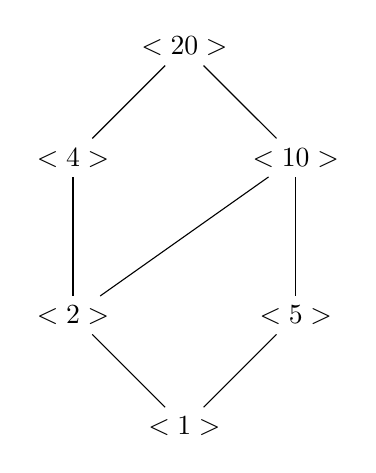
\begin{tikzpicture}[node distance=2cm]
			\node(20) {$<20>$};
			\node(10)  	[below right of=20] {$<10>$};
			\node(4)  	[below left of=20]  {$<4>$};
			\node(5) 	[below of=10] {$<5>$};
			\node(2)	[below of=4] {$<2>$};
			\node(1)	[below left of=5] {$<1>$};

			\draw(20) -- (10);
			\draw(20) -- (4);
			\draw(2) -- (4);
			\draw(2) -- (10);
			\draw(5) -- (10);
			\draw(2) -- (1);
			\draw(5) -- (1);
		\end{tikzpicture}
	\end{center}

	Here, the lines imply inclusion from top to bottom; that is
		\[<20>\subset<4>\subset<2>\subset<1>,\]
	for example. We won't spend a lot of time looking at subgroup lattices, but the idea of how to create them is more or less the same for our purposes.
\end{example}

Before we finish this section, we will look at some examples of groups and their subgroups.

\subsection*{The General Linear Group}
Numbers are just a small portion of the type of objects that sets can contain. One group that does not contain numbers is the General Linear Group, $(GL_{n}(\RR),\cdot)$, defined by
\[
	GL_{n}(\RR) = \left\{
	A=
	\left[
	\begin{array}{c c c c}
		a_{11} & a_{12} & \dots  & a_{1n} \\
		a_{21} & a_{22} & \dots  & a_{2n} \\
		\vdots & \vdots & \ddots & \vdots \\
		a_{n1} & a_{n2} & \dots  & a_{nn}
	\end{array}
	\right]
	:
	a_{i,j}\in\RR\text{ and } \det{(A)}\neq 0
	\right\}.
\]
In other words, it is the set of $n\times n$ invertible matrices with entries in $\RR$. The fact that every element in $GL_{n}(\RR)$ is invertible guarantees that inverses exist within the group. We know $I_{n}$ is contained within this group since its determinant is 1. Associativity is a little harder to prove, but it does indeed work. Hence, $GL_{n}(\RR)$ is in fact a group. The reason we point out this group is to mention one of its subgroups, the Special Linear Group $SL_{n}(\RR)$. We define this group by
\[
	\{A\in GL_{n}(\RR) : \det{(A)}=1\}.
\]
Let's show that $SL_{n}(\RR)$ is indeed a subgroup.

\begin{example}{Show $SL_{n}(\RR)$ is a subgroup.}
	We first need to find the identity within $SL_{n}(\RR)$. We know $\det{(I_{n})}=1$, so it lies within the Special Linear group. Next, we must verify that every element within $SL_{n}(\RR)$ has an inverse. Let $A\in SL_{n}(\RR)$. Then
	\[
		\det{(A^{-1})}=\det{(A)}^{-1}=1^{-1}=1,
	\]
	so the inverses exists within the subgroup. Finally, we must show that the group is closed. Let $A,B\in
	SL_{n}(\RR)$. Then
	\[
		\det{(AB)}=\det{(A)}\det{(B)}=1\cdot 1=1.
	\]
	Thus, we conclude that the group is closed, and therefore $SL_{n}(\RR)\leq GL_{n}(\RR)$
\end{example}

\subsection*{The Integers Multiplied by $n$}
We have seen that the group $\ZZ$ is a cyclic group generated by 1. It is true that there are other generators that generate subgroups of $\ZZ$ rather than $\ZZ$ itself. Specifically, we can take any $n\in\ZZ$ and examine the subgroup of $\ZZ$ generated by that element. We define this behavior with the notation
\[
	n\ZZ=\{nz:z\in\ZZ\} = <n>
\]
Our hope is that this forms a subgroup of $\ZZ$. It will turn out to be true, but let us look at a specific example.

\begin{example}{Consider the set $1727\ZZ$. Show that this is a subgroup of $\ZZ$, and that it is cyclic}
	Let's start with closure. Let $a,b\in 1727\ZZ$. Then $a=1727m$ and $b=1727n$ for some $n,m\in\ZZ$. Therefore
	\[
		a+b=1727m+1727n= 1727(m+n)\in 1727\ZZ,
	\]
	so $1727\ZZ$ is closed. We know the identity is inside of $1727\ZZ$ since $1727\cdot 0=0$. Finally, we need inverses to be inside the subgroup. Let $a\in 1727\ZZ$. Then
	\[
		a+-a= 1727n + (-1727n) = 0.
	\]
	from \cref{thm:cyclic_subgroup}, we know that it is cyclic since $\ZZ$ is cyclic.
\end{example}
The notion of multiplication of a group and an element of the group is a very important topic that we will discuss later.

\subsection*{The Center of a Group}
The next subgroup we will look at is called the center of a group. Recall that nowhere in the definition of group is it stated that the operation is commutative. To take care of this issue, we define a special subgroup called the center of a group. The formal definition is as follows.
\begin{definition}{Center of a Group}
	Let $G$ be a group. The center of $G$ is the group
	\[
		Z(G)=\{z\in G : zg=gz\ \forall g\in G\}.
	\]
	That is, the center of a group is the set of all elements that commute within $G$.
\end{definition}
It follows that if $G$ is an abelian group, then $Z(G)=G$. We claim that this is a subgroup.
\begin{example}{Show $Z(G)\leq G$}
	The identity is in the center since $eg = ge\ \forall g\in G$. Inverses require a little more work. Let $z\in Z(G)$. We need $z^{-1}g=gz^{-1}\ \forall g\in G$. Consider
	\begin{align*}
		zg         & =gz                \\
		z^{-1}(zg) & = z^{-1}(gz)       \\
		(z^{-1}z)g & = (z^{-1}g)z       \\
		g          & = (z^{-1}g)z       \\
		gz^{-1}    & = (z^{-1}g)zz^{-1} \\
		gz^{-1}    & = z^{-1}g.
	\end{align*}
	This is exactly what we needed, so we conclude that the group contains inverses. We will leave closure to you.
\end{example}

\section*{Problems}
\begin{compactenum}
    \item Give examples of the following groups, or explain why no such group exists
    \begin{compactenum}
        \item A cyclic group
        \item An abelian non-cyclic group
        \item A finite non-abelian group
        \item An infinite non-abelian group
        \item Two isomorphic groups of order 4
        \item Two non-isomorphic groups of order 4
        \item Three non-isomorphic groups of order 8
        \item A group and a normal subgroup of the group
        \item A group with a trivial center
        \item A non-abelian group with a trivial center
    \end{compactenum}
    \item Show the symmetric difference operator $\Delta$ is associative.\label{prob:sym_dif_ass}
    \item Let $G$ be a group and suppose $a,b\in G$. Show $ab=e\implies a=b^{-1}$.
    \item Show that $(\ZZ_{5}\setminus\{0\},\cdot)$ is a group, and construct its Cayley table. To what group does this look similar?
    \item Show $(\ZZ_{p},\cdot)$ is a group for any prime $p$.
    \item Is $\QQ$ cyclic? What about $\RR$? Why or why not?
    \item Let $G$ be a group and let $a\in G$ with $|a|=n\in\NN$. Show that for $m\in\NN$, $a^{m}=e\implies n\mid m$.
    \item Prove that the center of a group is closed.
    \item Define the Projective Special Linear Group, $PSL_{n}(\RR)$ as
    \[
        PSL_{n}(\RR)=\{A\in GL_{n}(\RR) : |\det{(A)}| = 1\}.
    \]
    Show $PSL_{n}(\RR)$ is a normal subgroup of $GL_{n}(\RR)$.
    \item Find the orders of the following elements in their respective groups.
    \begin{compactenum}
        \item 4 in $\ZZ_{20}$
        \item 8 in $\ZZ_{1000}$
        \item $(1\ 2\ 4)(3\ 6\ 5\ 7)(9\ 12)$ in $Sym_{12}$
    \end{compactenum}
    \item Find the order of $\fgroup{Sym_{3}}{<(1\ 2\ 3)>}$.
    \item Let
    \[
        \sigma=
        \left[
            \begin{array}{c c c c c}
                1 & 2 & 3 & 4 & 5\\
                2 & 4 & 1 & 5 & 3
            \end{array}
        \right]
        \qquad
        \tau=
        \left[
            \begin{array}{c c c c c}
                1 & 2 & 3 & 4 & 5\\
                3 & 5 & 2 & 4 & 1
            \end{array}
        \right]
    \]
    Find the following.
    \begin{compactenum}
        \item Cycle decomposition of $\sigma$ and $\tau$
        \item $\sigma\tau$
        \item $\tau\sigma$
        \item $\sigma^{2}$
        \item $\tau^{-1}$
        \item Transposition decomposition of $\tau$
        \item $\sgn(\sigma)$
    \end{compactenum}

    \item Let $H$ and $K$ be subgroups of $G$ and define $HK=\{hk:h\in H\land k\in K\}$
    \begin{compactenum}
        \item Show $H\cap K\leq G$.
        \item Show $H \cup K\leq G\iff (H\subset K)\lor (K\subset H)$.
        \item If $G$ is abelian, show $HK$ is a subgroup.
        \item Show that $K\normal G\implies HK\leq G$.
    \end{compactenum}
\end{compactenum}


\chapter{Rings and Fields}

Our study of groups only scratched the surface of the vast array of algebraic structures.
Here, we will examine two more algebraic structures that are more complex than groups.
Rings and fields are examples of structures with two operations, and as such require fine attention to detail in order to guarantee that the definitions hold.
We will begin with the simpler of the two structures, and a personal favorite of mine, rings.

\section{Introduction to Rings}

In the previous chapter, we looked in depth at the concept of a group.
Recall that groups are defined with one operation, which we called $*$; this need not alway be the case, however.
Groups are simple in this aspect especially when compared to other structures such as a Ring or a Field.
We will begin by defining a Ring.

\begin{definition}{Ring}
    Let $R$ be a set an let $+$ be the standard operation of addition and $\cdot$ be the standard operation of multiplication. We say $(R,+,\cdot)$ is a ring if
    \begin{enumerate}
        \item $(R,+)$ is an abelian group
        \item multiplication is associative
        \item multiplication distributes over addition.
    \end{enumerate}
\end{definition}

We can see that a ring is a much more complex structure than a group, and in fact it contains groups within it, similar to the idea that all squares are rectangles but not all rectangles are squares.
Like many of the structures in algebra, we have dealt with rings without even knowing it.
The groups $(\RR, +)$ and $(\RR^{*},\cdot)$ form a ring $(\RR, +, \cdot)$ when combined.
Note that the definition does \textit{not} require that $R$ be a group under multiplication; rather, we only need that multiplication is associative and that the distributive law holds.
It is this fact that allows us to construct a ring from one of our favorite groups.

\begin{example}{Show $\ZZ_{n}$ is a ring}
    We already know that $\ZZ_{n}$ is abelian under addition by the definition of the operation. We define multiplication in the context to be
    \[
        \overline{ab}=\overline{a}\overline{b}\equiv ab\mod n.
    \]
    Hence
    \begin{align*}
        (\overline{a}\overline{b})\overline{c} &= \overline{ab}\overline{c}\\
        &= \overline{abc}\\
        &= \overline{a}\overline{bc}\\
        &= \overline{a}(\overline{b}\overline{c}).
    \end{align*}
    The distributive law is trivial to show.
\end{example}

The concept of an identity element was crucial to our study of groups.
The identity was determined by the operation over the set, and it is no different for rings.
Here, we have two operations so we designate two identity elements, typically called 1 (for multiplication), and 0 (for addition).
We were also concerned with the concept of inverse elements, but we must be careful.
The additive inverse is guaranteed to us because of the fact that $(R,+)$ is a group, but we are not guaranteed a multiplicative inverse (although it is not impossible).



\part{Calculus}
\chapter{Real Analysis}

\chapter{Multi-variable Calculus}

\chapter{Complex Analysis}

\chapter{Ordinary Differential Equation}

\chapter{Partial Differential Equations}


\part{Statistics and Probability}
\chapter{Probability}

\chapter{Graph Theory and Combinatorics}

Graph theory is concerned with the study of structures we call graphs as well as topics within combinatorics.
By \textit{graph}, we don't mean graphs in the $f(x)$ sense; rather, we are talking about nodes connected by edges.
Often times, we represent these graphs with a picture involving dots and lines, representative of vertices and edges, respectively.
Throughout our discussion, keep in mind that we cannot rely on a picture for a proof, but it is very helpful to see the pictures to get an understanding of what's happening.

\section{Introduction to Graphs}

The idea of a graph is relatively simple but requires some prior ideas from the study of set theory.
Recall that given a set $A$, we can create what is known as the power set of a, $\mathcal{P}(A)$, consisting of all subsets of $A$.
We can extend this idea a little further but considering subsets of the power set of a given set.

\begin{definition}{Power-$k$ Set}
    Let $A$ be a finite set of order $n$ and let $k\in\NN$.
    The power-$k$ set of $A$, $\mathcal{P}_{k}(A)$, is the set of all subsets of $A$ with cardinality $k$.
\end{definition}

We get some nice relationships between the power-$k$ set and the power set of $A$.
First, note that $\mathcal{P}_{k}(A)\subset\mathcal{P}(A)\ \forall k$; even if $k > n$, we still have a subset of $\mathcal{P}(A)$ since $\mathcal{P}_{k}(A)=\emptyset$ in that case.
The power set can be expressed as a union of power-$k$ sets:
\[
    \mathcal{P}(A) = \bigcup_{k=1}^{n}\mathcal{P}_{k}(A).
\]
There are various other properties that follow, but our main purpose of introducing the power-$k$ set is to assist us in our definition of a graph.

\begin{definition}{Graph}
    Let $V$ be a finite set and let $E\subset\mathcal{P}_{2}(V)$.
    The pair $(V,E)$ is called a graph, with the vertex set $V$ and the edge set $E$.
\end{definition}

This is our main definition to keep in mind throughout this entire chapter.
We may often see pictures of graphs drawn with dots and lines, but it is the pair of sets that truly defines the structure.
We can, and usually do, prefer to draw graphs from the provided sets in order to determine various properties.

\begin{example}{Let $V=\{a,b,c\}$ and $E=\{\{a,b\},\{b,c\}\}$. Draw a representation of this graph.}
    We ought to first determine whether or not $(V,E)$ actually is a graph.
    We require $E$ to have two main properties:

    \begin{enumerate}
        \item Every element of every set within $E$ is an element of $V$.
        \item $E\subset\mathcal{P}_{2}{V}$.
    \end{enumerate}

    Indeed, both these properties hold, so $(V,E)$ is a graph.
    We could draw infinitely many representations of $(V,E)$; here is one such.
    \begin{center}
        \begin{tikzpicture}[node distance=1cm]
            \node(a) {a};
    		\node(b) [below left of=a] {b};
    		\node(c) [below right of=a] {c};

    		\draw(a) -- (b);
    		\draw(b) -- (c);
        \end{tikzpicture}
    \end{center}
    The pairs within the $E$ represent the vertices which share an edge; the values within $V$ represent the vertices themselves.
\end{example}

One key fact to note is that the definition does not require the pairs within $E$ to be ordered; if they are ordered, then we have what is called a directed graph.
We also don't have any repeated edges (if we do, we have a multigraph), and no vertex can share an edge to itself (called a pseudograph)
We will look at directed graphs in depth later, but for now we will consider the non-directed case.

The next few pages will concern a whole slew of definitions.
The terminology here is not always standard, but it is what we will go with for the rest of our discussion on graphs.

\begin{definition}{Order}
    Suppose $G$ is a graph. Then the order of $G$ is $ord(G)=|V(G)|$.
\end{definition}
\begin{definition}{Size}
    Suppose $G$ is a graph. Then the size of $G$ is $size(G)=|E(G)|$.
\end{definition}

These terms are more for convenience. The next few are actually useful.

\begin{definition}{Degree}
    Let $v\in V(G)$. The degree of $v$ in $G$, $deg_{G}(v)$, is the number of edges incident with $v$.
    We often write $deg(v)$ if the context of the graph is obvious.
\end{definition}

The degree of a vertex tells us how many edges come out of the vertex.
As it so happens, we actually know how large this number can be: $ord(G) - 1$.
This makes sense intuitively; a vertex can have no duplicate edges and no edges to itself, so the max number of edges a given vertex can have is an edge to every other vertex in the graph.
If every vertex has this property, we call the graph \textit{complete}.

\begin{definition}{Complete}
    Let $G$ be a graph and let $n=ord(G)$. We call $G$ complete if $\forall\ v\in V(G),\ deg(v)=n-1$. Since these graphs are unique, we say $G=K_{n}$, meaning the complete graph on $n$ vertices.
\end{definition}

The concept of graph equality is something that we discuss further in a little bit.
For now, we are ready for our first theorem.

\begin{theorem}{}
    Suppose $G$ is a graph. Then
    \[
        \sum_{v\in V(G)}deg(v) = 2\ size(G).
    \]
\end{theorem}
\begin{proof}
    We can show this via induction. Suppose $size(G)=0$. Then $2\ size(G)=2\cdot0=0$.
    Since $size(G)=0$, $deg(v)=0\ \forall v\in V(G)$, so the sum over the degrees is also 0.
    Hence, we may assume for all graphs $H$ with $n$ edges,
    \[
        \sum_{v\in V(H)}deg_{H}(v) = 2n.
    \]
    Assume $G$ has $n+1$ edges. We must show
    \[
        \sum_{v\in V(G)}deg(v)=2(n+1).
    \]
    Let $H$ be a graph such that $V(H)=V(G)$ and $E(H)=E(G)\setminus ab$ for some $ab\in E(G)$. Then
    \[
        \sum_{v\in V(H)}deg_{H}(v)=2n\implies\sum_{v\in V(G)}deg_{H}(v)=2n.
    \]
    Since $ab\in E(G),\ \exists v_{1},v_{2}\in V(G)$ which are incident with $ab$.
    Hence $deg_{H}(v_{1})+1=deg_{G}(v_{1})$ and $deg_{H}(v_{2})+1=deg_{G}(v_{2})$.
    Note that for all other vertices in $v\in V(G)$, $deg_{H}(v)=deg_{G}(v)$.
    Then
    \[
        \sum_{v\in V(G)}deg_{H}(v)=-2+\sum_{v\in V(G)}deg_{G}(v).
    \]
    By the inductive hypothesis, we have
    \[
        2n=\left( \sum_{v\in V(G)}deg_{G}(v) \right) - 2\implies
        2(n+1)=\sum_{v\in V(G)}deg_{G}(v).
    \]
\end{proof}

Induction is a very common proof technique that we will encounter throughout or study of graphs; the strategy of creating a new graph with properties of our old graph is also a very useful technique.

\section{Walks, Paths, and Trails}

The topics covered in this section address the ways we can traverse graphs.
In our study, we have the freedom to move from any vertex to any other vertex as long as there is an edge between them.
The strategies we use to move around a graph form the theory of walks, paths, and trails.

\begin{definition}{Walk}
	Suppose $G$ is a graph. We say a finite sequence of vertices $v_{1},v_{2},\dots,v_{k}$ is a walk of length $k$ provided that $v_{i}v_{i+1}\in E(G)$ for all $1\leq i\leq k$. If $v_{1}=v_{k}$, then we say the walk is closed.
\end{definition}

In other words, a sequence of vertices is a walk if we can always move along a single edge to the next vertex in the sequence.
We have several ways to write walks; we can use set notation $\{a,b,c,d\}$ or simply write the vertices in the order they appear, $abcd$, if it is obvious to do so.

\begin{example}{}

	\begin{minipage}{0.3\textwidth}
		\begin{tikzpicture}[node distance=1cm]
			\node(a) {a};
			\node(b) [above right of=a] {b};
			\node(c) [below right of=b] {c};
			\node(d) [below of=c] {d};
			\node(e) [below left of=d] {e};

			\draw(a) -- (b);
			\draw(b) -- (c);
			\draw(c) -- (d);
			\draw(b) -- (d);
			\draw(d) -- (e);
		\end{tikzpicture}
	\end{minipage}
	\begin{minipage}[t]{0.65\textwidth}
        \vspace{-1.2cm}
		In this graph, $abde$ and $abcba$ form walks, but $ade$ does not since there is $ad\notin E(G)$.
        Note that we can repeat vertices if need be.
	\end{minipage}

\end{example}

Walks are simplistic in their construction since we can move anywhere in the graph where there is an edge.
The more interesting idea here is a walk where no vertices are repeated.

\begin{definition}{Path}
    Let $W$ be a walk in a graph $G$. If $W$ contains no repeated vertices, then we call $W$ a path. If we include the edge $v_{k}v_{1}$, provided that it exists, the we call the path closed, or a cycle.
\end{definition}

Paths concern vertices, but there is an analogous idea for edges.

\begin{definition}{Trail}
    If all edges in a walk are distinct, then it is called a trail.
\end{definition}

When talking about walks and paths, we say the length of the walk is the number of edges in the walk.
If the path is closed, then we count the missing edge in the path as part of the length.
With these definitions in mind, we now have enough to build our first theorem.

\begin{theorem}{}
    Let $G$ be a graph and let $A$ be a walk in $G$. If $A$ is not a trail, then $A$ is not a path.
\end{theorem}

We won't prove this here, but note that the contrapositive holds (and is a little more pleasing to read)

\begin{theorem}{}
    If $A$ is a path, then $A$ is a trail.
\end{theorem}

Again, we won't prove this, but it is important to keep in mind. The next theorem, however, is a little more worthwhile to prove.

\begin{theorem}{}
    Suppose $G$ is a graph and let $u,v\in V(G)$ be distinct. Then every $uv$ walk contains a $uv$ path.
\end{theorem}
\begin{proof}
    Let $A$ be a $uv$ walk, and assume $A$ has length 1. Hence, $u$ and $v$ are the only vertices in the walk, so $A$ is a path. Assume that all $uv$ walks of length $l$ contain a $uv$ path.
    We must show that for a $uv$ walk $A$ of length $l+1$ contains a $uv$ path.
    Since $A$ is a walk, we may name the vertices in $A$:
    \[
        A = v_{1}v_{2}\dots v_{k}
    \]
    with $u=v_{1}$ and $v=v_{k}$.
    If $A$ is a $uv$ path then we are done, so assume that $A$ is not a path.
    Then $\exists i\neq j \suchthat v_{i}=v_{j}$.
    Define $B$ to be a walk such that
    \[
        B = v_{1}v_{2}\dots v_{i}v_{j+1}v_{j+2}\dots v_{k}.
    \]
    We have removed at least one edge from $A$ to create $B$, so the length of $B$ is less than or equal to $l$.
    By the inductive hypothesis, we have that $B$ contains a $uv$ path $C$.
    Hence if $C$ is contained in $B$ and $B$ is contained in $A$, then $C$ is contained in $A$, so $A$ contains a $uv$ path.
\end{proof}

This is a very important result since it allows us to find a $uv$ path in any $uv$ walk.

\section{Types of Graphs}

A typical graph probably does not have any special characteristics that set that graph apart from others.
There are, however, a whole slew of graphs that are recognized separately from a typical graph.
Among these are complete graphs and bipartite graphs, which we will examine here.

\subsection*{Complete Graphs}

To grasp the concept of a complete graph, we must first understand the idea of connectedness.
We will, as is common in graph theory, begin with a definition.

\begin{definition}{Connected}
	A graph $G$ is called connected if for every pair of vertices $u,v\in V(G)$, there is a $uv$ walk in $G$.
	$G$ is called disconnected if it is not connected.
\end{definition}

In other words, we can get from any vertex to any other vertex in the graph no matter what.
It is especially important to realize that pictures can deceive us here, as the next example will show.

\begin{example}{Determine if the following graph is connected}
	\begin{center}
		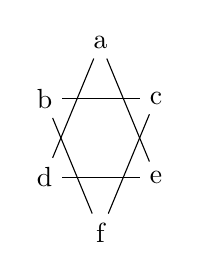
\begin{tikzpicture}[node distance=1cm]
			\node(a) {a};
			\node(b) [below left of=a] {b};
			\node(c) [below right of=a] {c};
			\node(d) [below of=b] {d};
			\node(e) [below of=c] {e};
			\node(f) [below right of=d] {f};

			\draw(a) -- (d);
			\draw(d) -- (e);
			\draw(e) -- (a);
			\draw(b) -- (f);
			\draw(f) -- (c);
			\draw(b) -- (c);
		\end{tikzpicture}
	\end{center}

	As it turns out, this graph is not connected, since there is no $ab$ path, even though the two cycles are drawn on top of each other.
\end{example}

In the above example, we can see two cycles, $adea$ and $bcfb$.
These two cycles are completely disjoint from each other; we cannot start on one and get to the other.
Hence, the two cycles actually form smaller graphs themselves. We call them \textit{subgraphs}

\begin{definition}{Subgraph}
	Suppose $G$ is a graph, and let $H$ be a graph such that $V(H)\subset V(G)$ and $E(H)\subset E(G)$.
	Then $H$ is a subgraph of $G$, denoted by $H\leq G$.
\end{definition}

In our case, we actually have two disconnected subgraphs who together from $G$.
If this is the case, we can take the concept of subgraphs a step further.

\begin{definition}{Connected Component}
	Suppose $G$ is a graph, and let $H$ be a graph such that $H\leq G$. Then $H$ is called a connected component if
	\begin{enumerate}
		\item $H$ is connected
		\item $v\in V(H)$ and $u\in V(G)\setminus V(H) \implies$ there is no $uv$ path in $G$.
	\end{enumerate}
\end{definition}

This is exciting, since we can now say $adea$ and $bcfb$ form connected components of $G$.
Not all graphs will contain connected components, however; if this is the case, we might be interested in trying to create connected components by removing either a vertex or an edge from the graph.
If we can accomplish this, then we call the removed vertices or edges by special names.

\begin{definition}{Cut Vertex}
	Let $G$ be a graph with $v\in V(G)$. Then $v$ is called a cut vertex of $G$ if the graph formed by removing $v$, $G-v$, has more connected components that $G$.
\end{definition}

We need to be a little cautious when we say \textit{remove $v$}; removing a vertex requires us to remove all the edges incident with that vertex as well.

\begin{example}{Determine the cut vertices of the following graph.}
	\begin{center}
		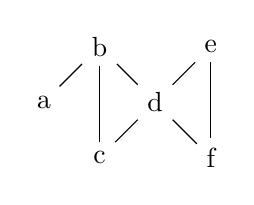
\begin{tikzpicture}[node distance=1cm]
			\node(a) {a};
			\node(b) [above right of=a] {b};
			\node(c) [below right of=a] {c};
			\node(d) [above right of=c] {d};
			\node(e) [above right of=d] {e};
			\node(f) [below right of=d] {f};

			\draw(a) -- (b);
			\draw(b) -- (c);
			\draw(b) -- (d);
			\draw(c) -- (d);
			\draw(d) -- (e);
			\draw(d) -- (f);
			\draw(e) -- (f);
		\end{tikzpicture}
	\end{center}

	We need to identify vertices that create connected components upon their removal. The vertex $d$ does the job here, since $G-d$ looks like

	\begin{center}
		\begin{tikzpicture}[node distance=1cm]
			\node(a) {a};
			\node(b) [above right of=a] {b};
			\node(c) [below right of=a] {c};
			\node(d) [above right of=c] {};
			\node(e) [above right of=d] {e};
			\node(f) [below right of=d] {f};

			\draw(a) -- (b);
			\draw(b) -- (c);
			\draw(e) -- (f);
		\end{tikzpicture}
	\end{center}
	where one connected component is given by the vertices $abc$ and the other by the vertices $ef$.
	There is another vertex that works here: $b$. Note that a single vertex is connected by definition, and $G-b$ looks like
	\begin{center}
		\begin{tikzpicture}[node distance=1cm]
			\node(a) {a};
			\node(b) [above right of=a] {};
			\node(c) [below right of=a] {c};
			\node(d) [above right of=c] {d};
			\node(e) [above right of=d] {e};
			\node(f) [below right of=d] {f};

			\draw(c) -- (d);
			\draw(d) -- (e);
			\draw(d) -- (f);
			\draw(e) -- (f);
		\end{tikzpicture}
	\end{center}

	where $a$ is one connected component and $c,d,e,$ and $f$ are in the other connected component.
\end{example}

Similarly, we have a definition for edges that accomplish this task.
Removal of edges is simpler than vertices, however, since we need not worry about the vertices incident with the edge.

\begin{definition}{Bridge}
	Let $G$ be a graph with $e\in E(G)$. Then $e$ is called a bridge of $G$ if the graph formed by removing $e$, $G-e$, contains more connected components than $G$.
\end{definition}

Vertices seem to be the more interesting object to remove from a graph, so we will focus on them a little more than edges.
We have a special name for the set of vertices that are cut verticies.

\begin{definition}{Cut Set}
	Let $G$ be a graph and let $S\subset V(G)$. $S$ is called a cut set of $G$ if the graph with vertex set $V(G)\setminus S$ is disconnected.
\end{definition}

In other words, if we remove all the cut vertices from a graph, we expect that graph to be disconnected.
Indeed, this makes intuitive sense, since any graph with more than one connected component is disconnected, and cut vertices create connected components.
With the notion of cut set, we can finally introduce completeness of graphs.

\begin{definition}{Complete}
	Let $G$ be a graph. $G$ is called complete if and only if $G$ has no cut sets.
	We denote a complete graph by $K_{n}$ where $n=ord(G)$.
\end{definition}

A complete graph consists of $n$ vertices that have every edge possible; hence removing one of the vertices isn't a problem since every other vertex is still connected to any other vertex in the graph.

\begin{example}{}
	The following are examples of complete graphs.
	\begin{center}
		\begin{tabular}{c c c}
			\begin{tikzpicture}[node distance=1cm]
                \node(a) {a};
                \node(b) [left of=a] {b};

                \draw(a) -- (b);
			\end{tikzpicture} &
			\begin{tikzpicture}[node distance=1cm]
                \node(a) {a};
                \node(b) [below right of=a] {b};
                \node(c) [above right of=b] {c};

                \draw(a) -- (b);
                \draw(b) -- (c);
                \draw(c) -- (a);
			\end{tikzpicture} &
			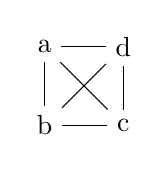
\begin{tikzpicture}[node distance=1cm]
                \node(a) {a};
                \node(b) [below of=a] {b};
                \node(c) [right of=b] {c};
                \node(d) [above of=c] {d};

                \draw(a) -- (b);
                \draw(a) -- (c);
                \draw(a) -- (d);
                \draw(b) -- (c);
                \draw(b) -- (d);
                \draw(c) -- (d);
			\end{tikzpicture}\\
            $K_{2}$ & $K_{3}$ & $K_{4}$
		\end{tabular}
	\end{center}
\end{example}

\subsection*{Bipartite Graphs}

The next type of graph we will study is called a bipartite graph.
Bipartite graphs are unique in that they can be partitioned into two sets that contain disconnected vertices.

\begin{definition}{Bipartite}
    Let $G$ be a graph and let $W\subset V(G)$. $G$ is called bipartite if for every edge in $uv\in E(G)$, either $u\in W$ and $v\in V(G)\setminus W$, or $u\in V(G)\setminus W$ and $v\in W$.
\end{definition}


\chapter{Statistics}


\part{Case Studies}
\chapter{Linear Algebra}

\chapter{p-adic Analysis}

The p-adic numbers combine various ideas from both analysis and algebra, making them the perfect application to stidy for both those fields.


\begin{appendices}
	\chapter{Major Theorems}

    \chapter{Important Definitions}
Some text

	\chapter{Tests for Convergence}
This appendix outlines the basic tests for convergence we can use in $\RR$. For an in depth look, refer to the appropriate chapter concerning the analysis of the set you want.

\section{Series in $\RR$}

\subsection*{Geometric Series}
\[
	\text{Given }\sum_{n=1}^{\infty}ar^{n-1}\text{ then }
	\begin{cases}
		|r| < 1 \implies \text{ convergence to } \frac{a}{1-r} \\
		|r| \geq 1 \implies \text{ divergence}
	\end{cases}
\]

\subsection*{P-Series}
\[
	\text{Given }\sum_{n=1}^{\infty}\frac{1}{n^{p}}\text{ then }
    \begin{cases}
        p > 1 \implies \text{ the series converges}\\
        p \leq 1 \implies \text{ the series diverges}
    \end{cases}
\]

\subsection*{Telescoping Series}
\begin{gather*}
    \text{Given }\sum_{n=1}^{\infty}\left(\frac{1}{n}-\frac{1}{n+1}\right)\text{ then}\\
    \lim_{n\to\infty}\left(\frac{1}{n}-\frac{1}{n+1}\right)=L <\infty\implies\text{ convergence at } L
\end{gather*}

\subsection*{Divergence Test}
\begin{gather*}
    \text{Given } \sum_{n=1}^{\infty}a_{n}\text{ then}\\
    \lim_{n\to\infty}a_{n}\neq0\implies\text{ divergence}
\end{gather*}

\subsection*{Integral Test}
\[
\text{Given }\sum_{n=1}^{\infty}a_{n},
\]
Let $f(n)=a_{n}$. If $f(n)$ is \textbf{Continuous}, \textbf{Positive}, and \textbf{Decreasing}, then
\[
\sum_{n=1}^{\infty}a_{n} \text{ converges } \iff \int_{0}^{\infty}f(n)\text{dn}\text{ exists.}
\]

\subsection*{Comparison Test}
\[
    \text{Given }\sum_{n=1}^{\infty}a_{n},
\]
choose $b_{n}$ such that
\[
    \sum_{n=1}^{\infty}a_{n}\text{ is similar to }\sum_{n=1}^{\infty}b_{n}.
\]
Then
\begin{gather*}
    \sum_{n=1}^{\infty}b_{n} \text{ converges and } a_{n} < b_{n}\ \forall n\in\NN\implies a_{n}\text{ converges}\\
    \sum_{n=1}^{\infty}b_{n} \text{ diverges and } a_{n} > b_{n}\ \forall n\in\NN\implies a_{n}\text{ diverges}\\
\end{gather*}

\subsection*{Limit Comparison Test}
\[
\text{Given }\sum_{n=1}^{\infty}a_{n},
\]
choose $b_{n}$ such that
\[
    \sum_{n=1}^{\infty}a_{n}\text{ is similar to }\sum_{n=1}^{\infty}b_{n},
\]
and consider
\[
    \lim_{n\to\infty}\frac{a_{n}}{b_{n}} = L.
\]
Then
\begin{gather*}
    L \geq 0 \text{ and } \sum_{n=1}^{\infty}b_{n}\text{ converges }\implies\sum_{n=1}^{\infty}a_{n}\text{ converges}.\\
    L > 0\text{ and }\sum_{n=1}^{\infty}b_{n}\text{ diverges }\implies\sum_{n=1}^{\infty}a_{n}\text{ diverges}.\\
    L\to\infty\text{ and }\sum_{n=1}^{\infty}b_{n}\text{ diverges }\implies\sum_{n=1}^{\infty}a_{n}\text{ diverges}.
\end{gather*}

\subsection*{Ratio Test}
\[
\text{Given }\sum_{n=1}^{\infty}a_{n},
\]
consider
\[
\lim_{n\to\infty}\frac{a_{n+1}}{a_{n}}=L.
\]
Then
\begin{gather*}
    L < 1 \implies a_{n}\text{ converges}.\\
    L > 1 \implies a_{n}\text{ diverges}.
\end{gather*}

\subsection*{Root Test}
\[
\text{Given }\sum_{n=1}^{\infty}a_{n},
\]
consider
\[
\lim_{n\to\infty}\sqrt[n]{a_{n}}=L.
\]
\begin{gather*}
    L < 1 \implies a_{n}\text{ converges}.\\
    L > 1 \implies a_{n}\text{ diverges}.
\end{gather*}

\subsection*{Alternating Series Test}
\[
\text{Given }\sum_{n=1}^{\infty}(-1)^{n-1}a_{n},
\]
then
\[
|a_{n+1}|\leq|a_{n}| \text{ and } \lim_{n\to\infty}|a_{n}|=0 \implies a_{n}\text{ converges.}
\]

\section{Series in $\CC$}

\section{Power Series in $\QQ_{p}$}

    \chapter{Common Riemann Integration Techniques}

    \chapter{Solutions to Selected Problems}

\end{appendices}

\end{document}
